\newpage
\section{tauNM distribution}
\label{appendix:tauNM}

\begin{figure*}[h!tpb]
\begin{center}
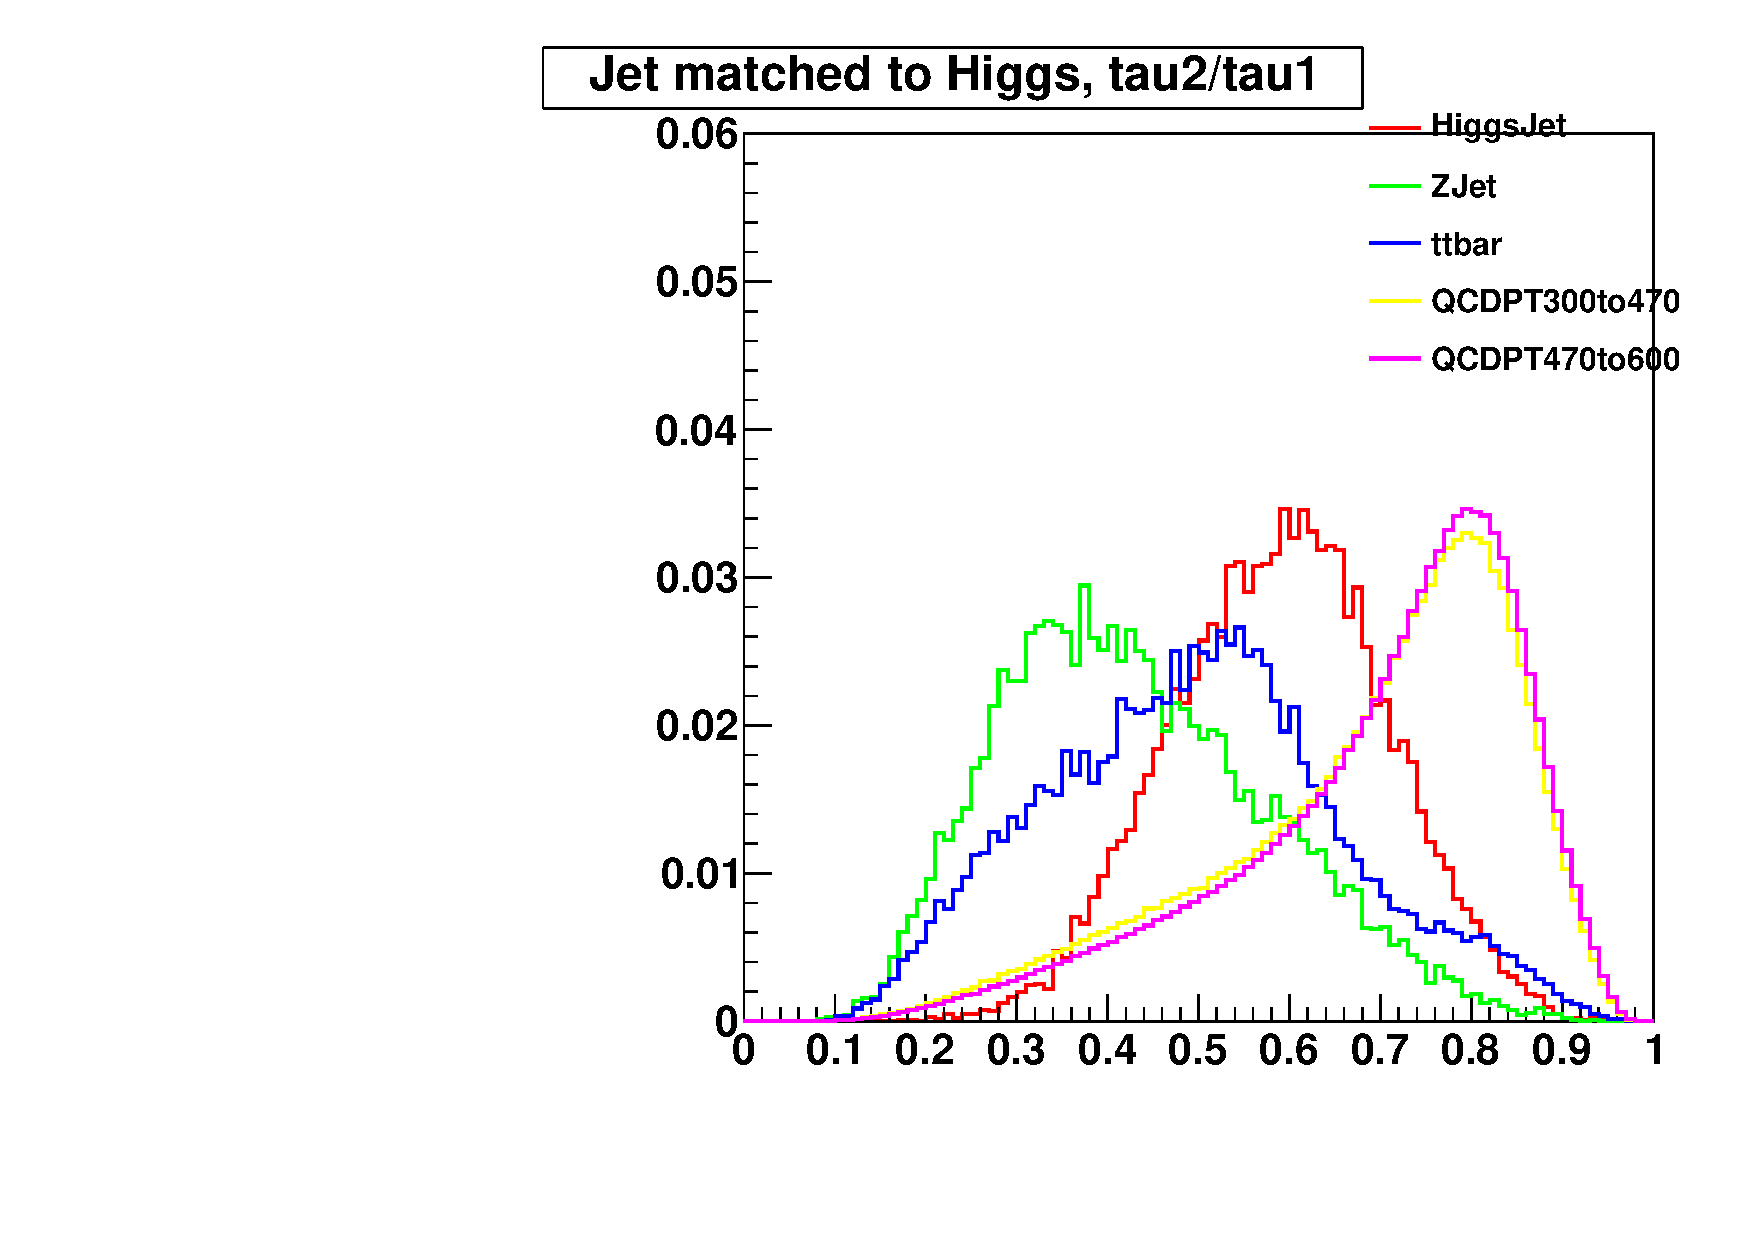
\includegraphics[width=0.49\textwidth]{HqqqqZqqfigs/tauNM/Tau21Pre.pdf}
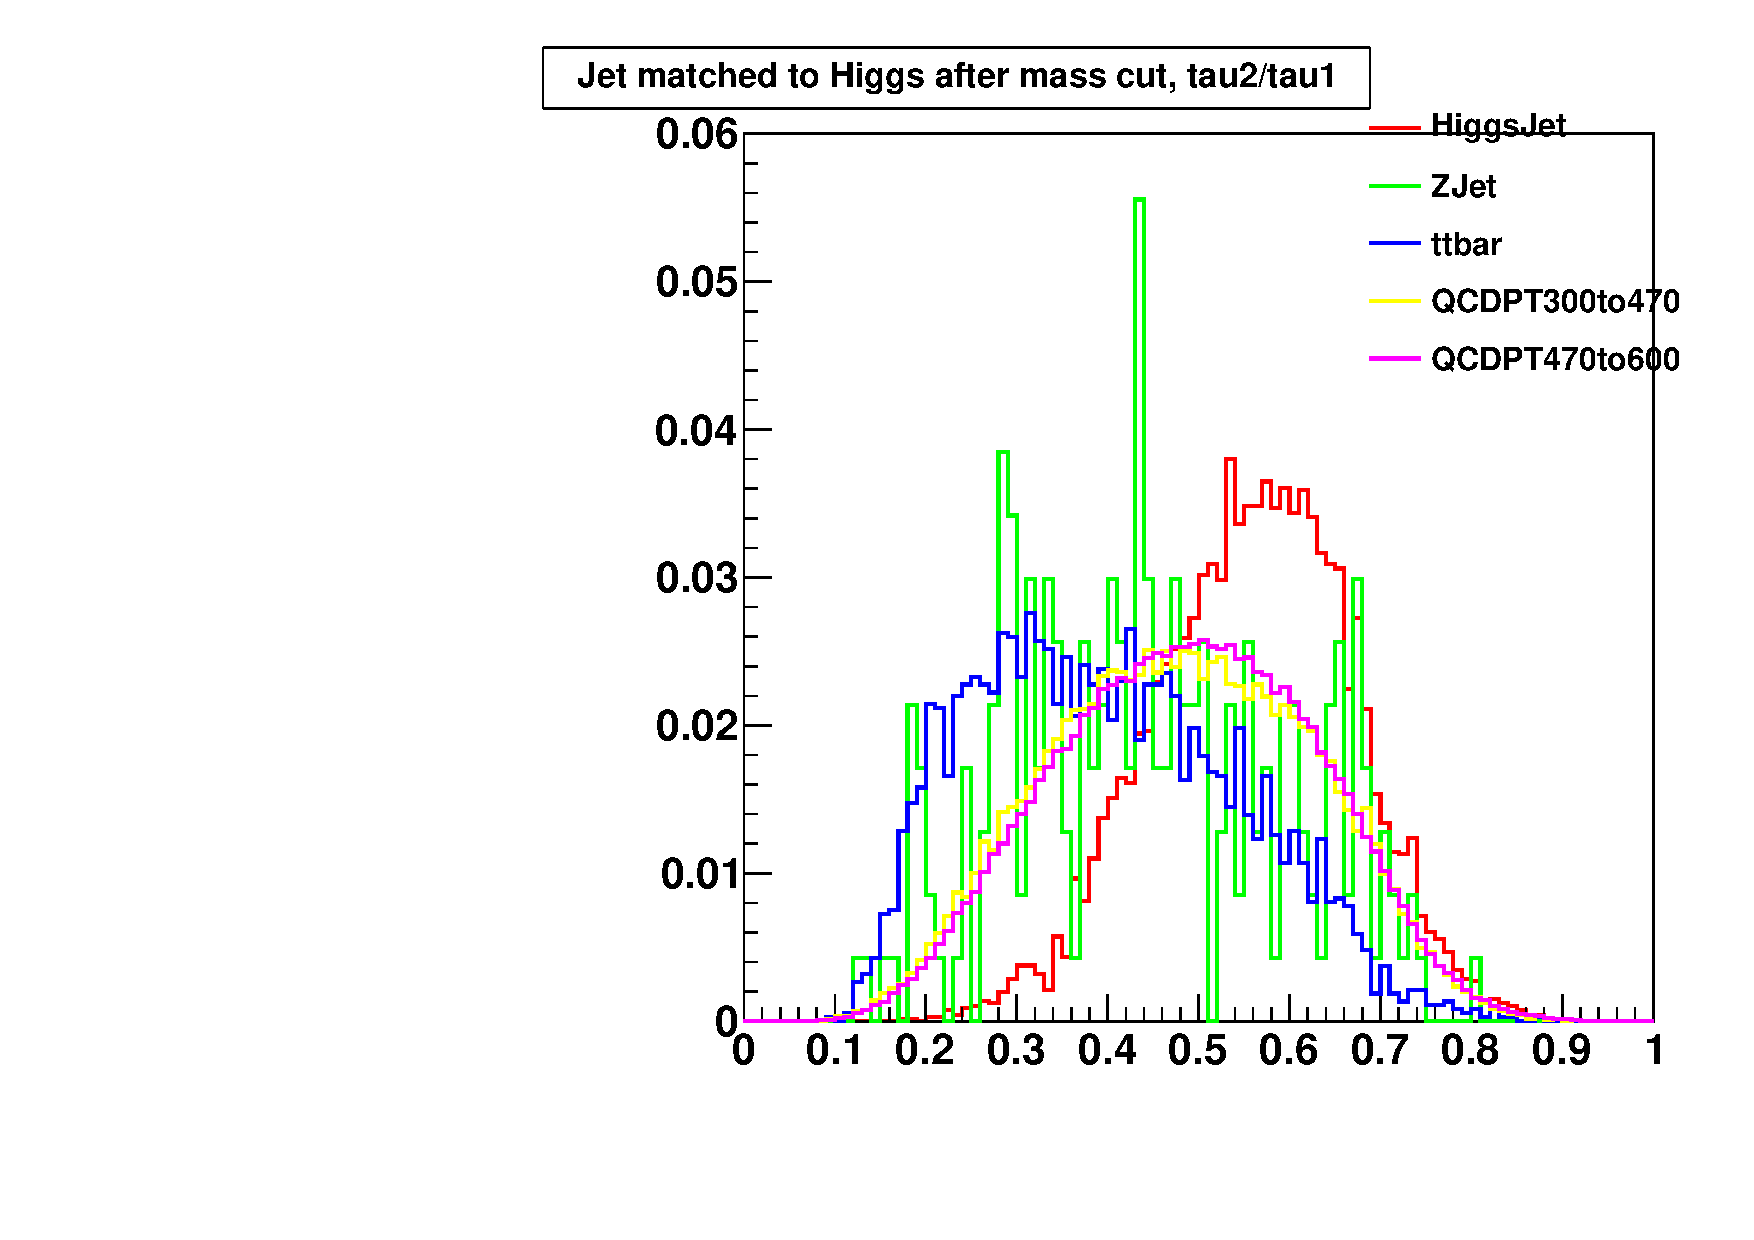
\includegraphics[width=0.49\textwidth]{HqqqqZqqfigs/tauNM/Tau21After.pdf}
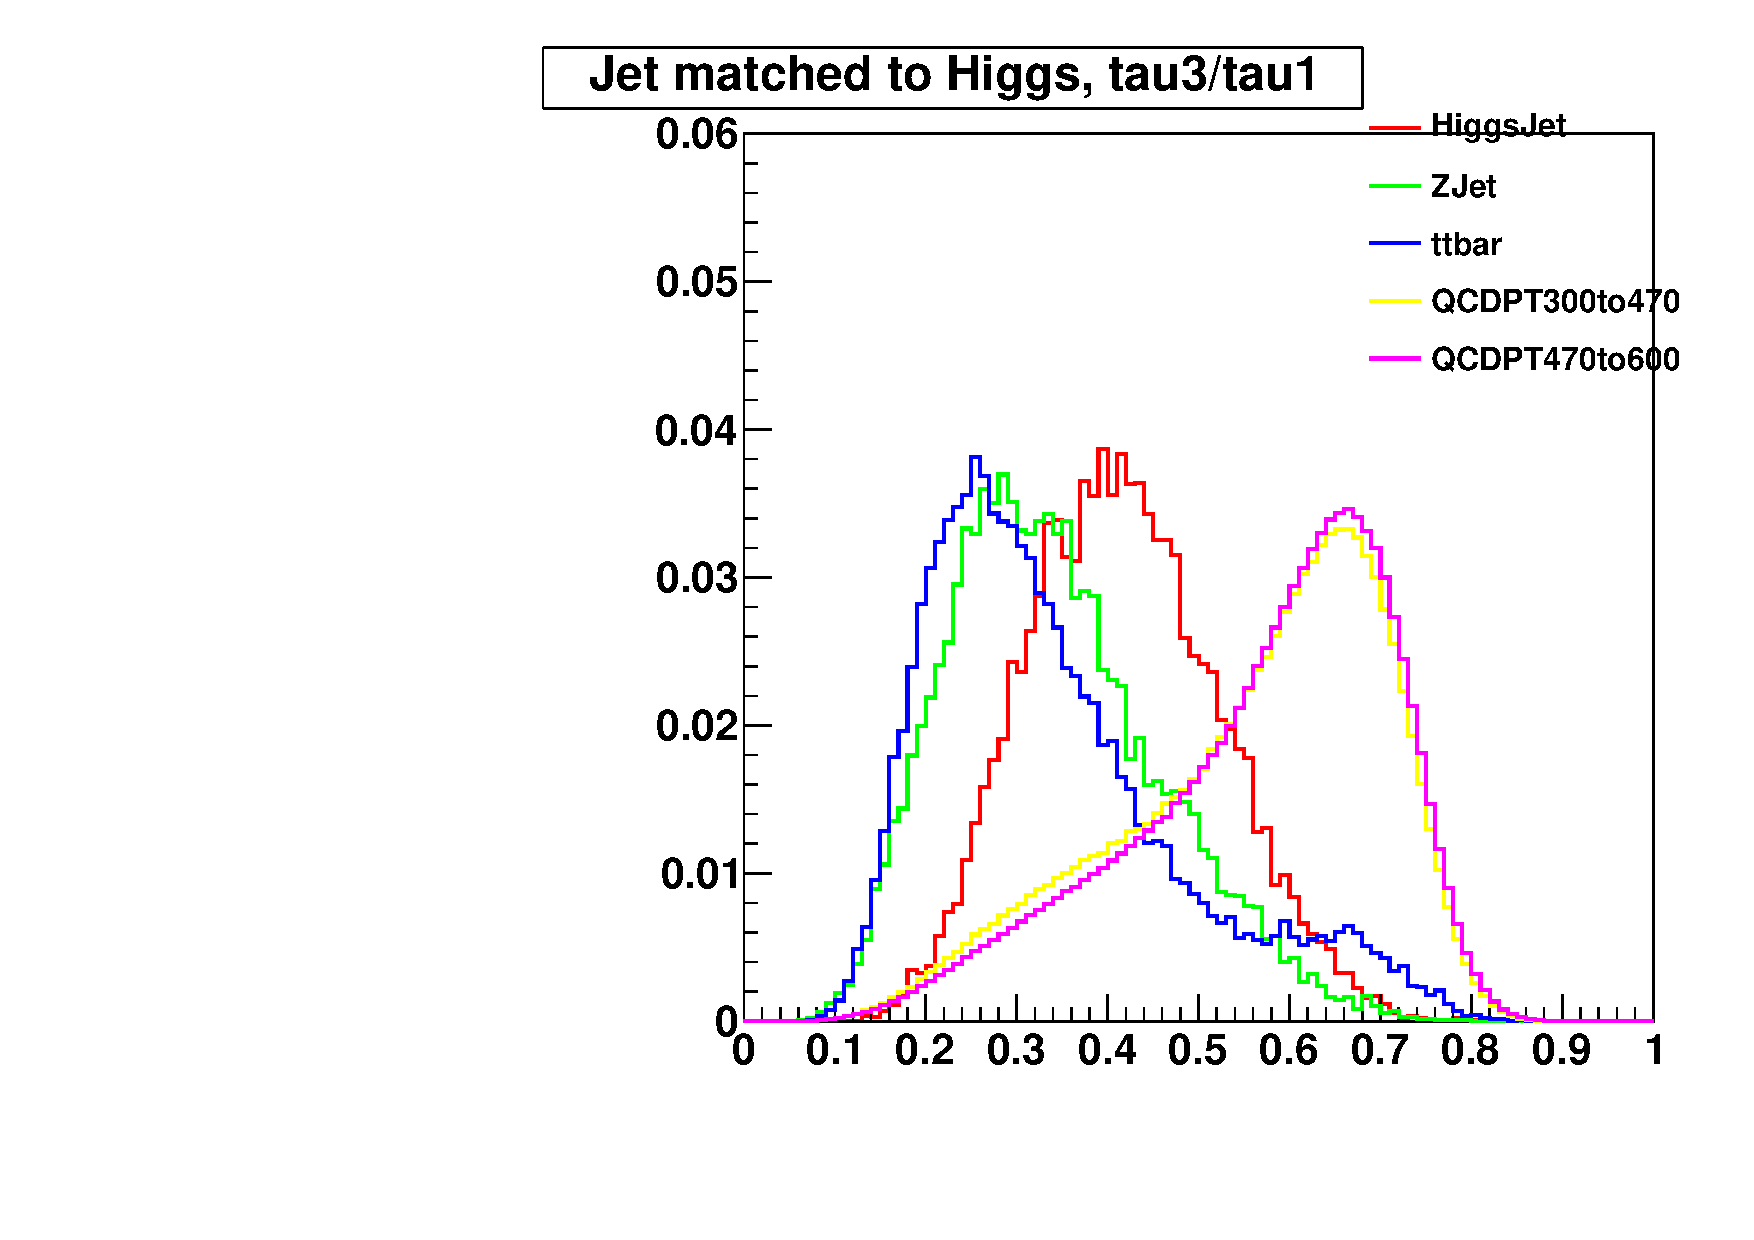
\includegraphics[width=0.49\textwidth]{HqqqqZqqfigs/tauNM/Tau31Pre.pdf}
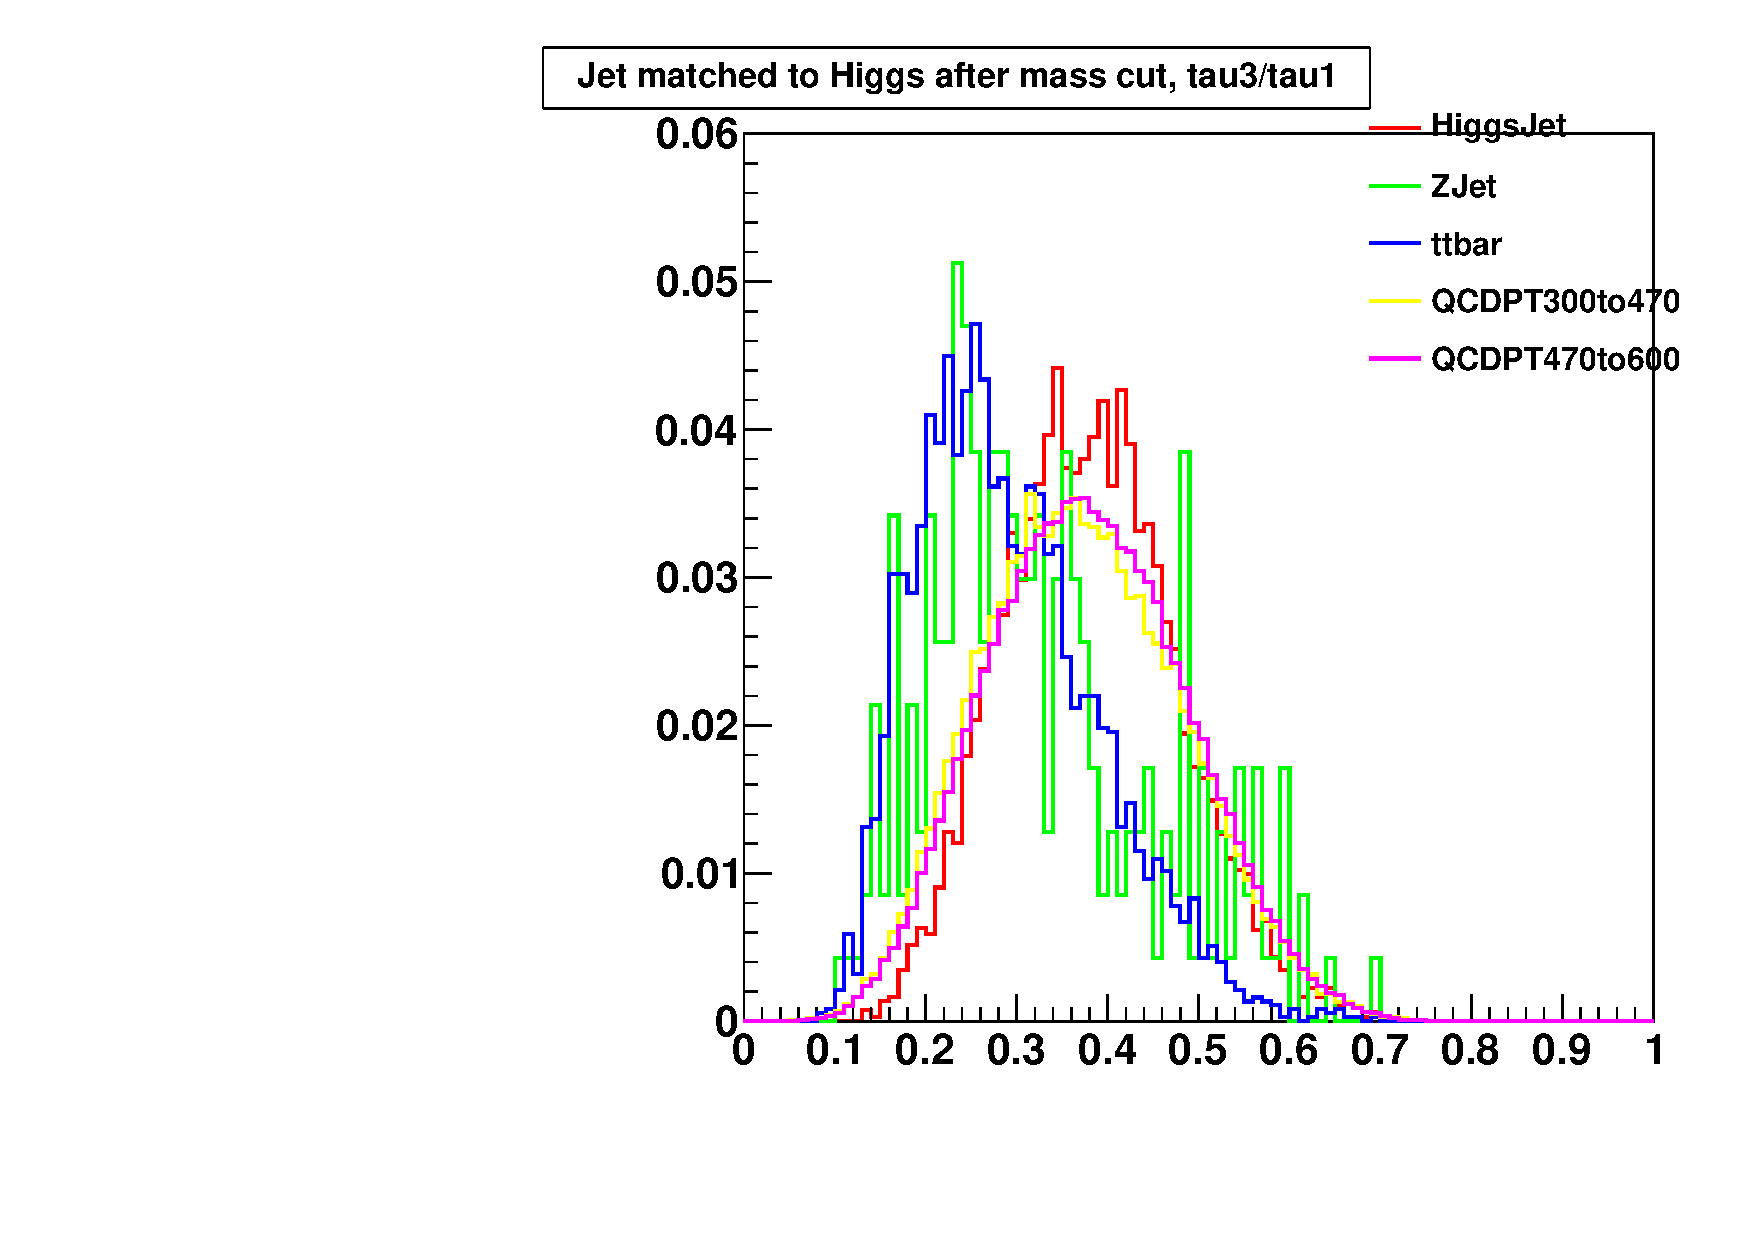
\includegraphics[width=0.49\textwidth]{HqqqqZqqfigs/tauNM/Tau31After.pdf}
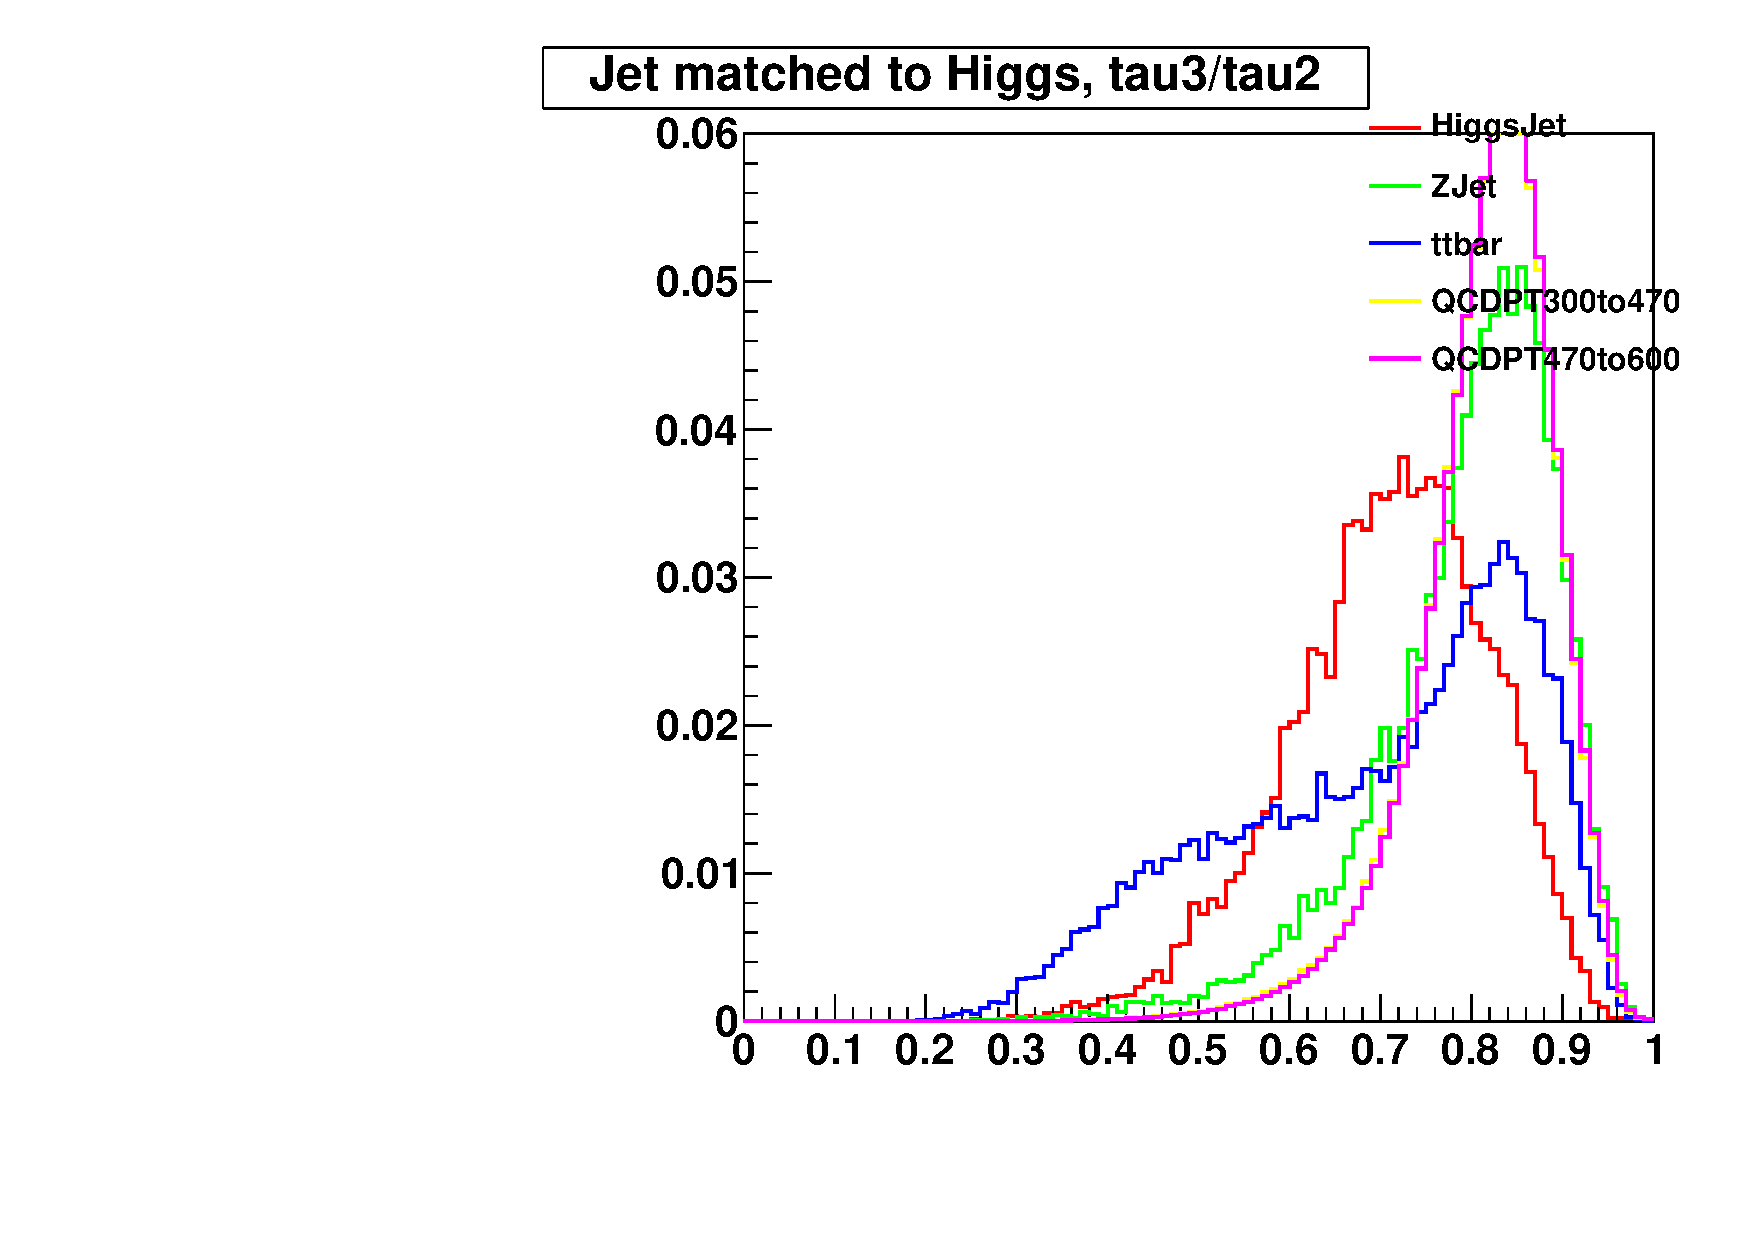
\includegraphics[width=0.49\textwidth]{HqqqqZqqfigs/tauNM/Tau32Pre.pdf}
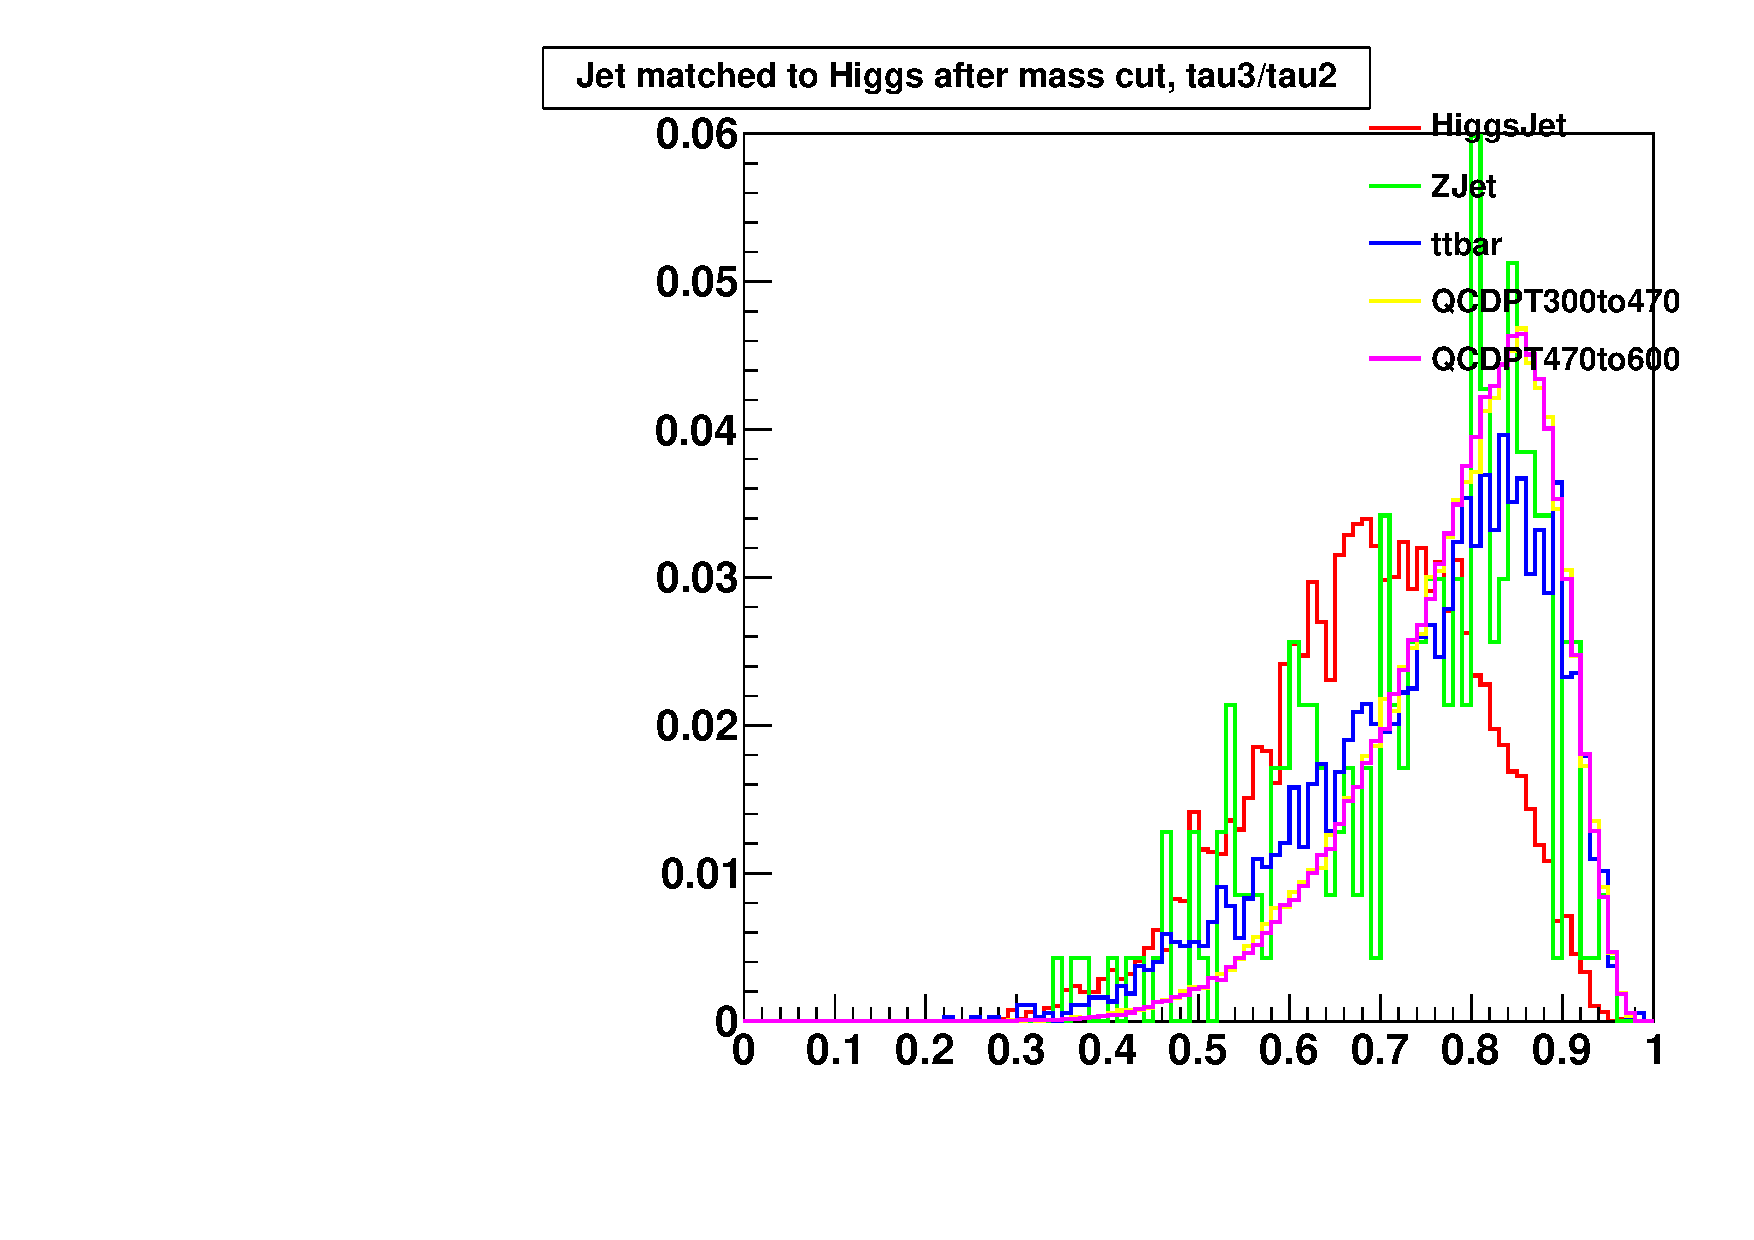
\includegraphics[width=0.49\textwidth]{HqqqqZqqfigs/tauNM/Tau32After.pdf}
\end{center}
\caption{
list of tauNM plots between Higgs genJet and Z genJet, hadronic top and QCD.
Signal used is 2 TeV Z'.  
}
\label{fig:tauNM1}
\end{figure*}

\begin{figure*}[h!tpb]
\begin{center}
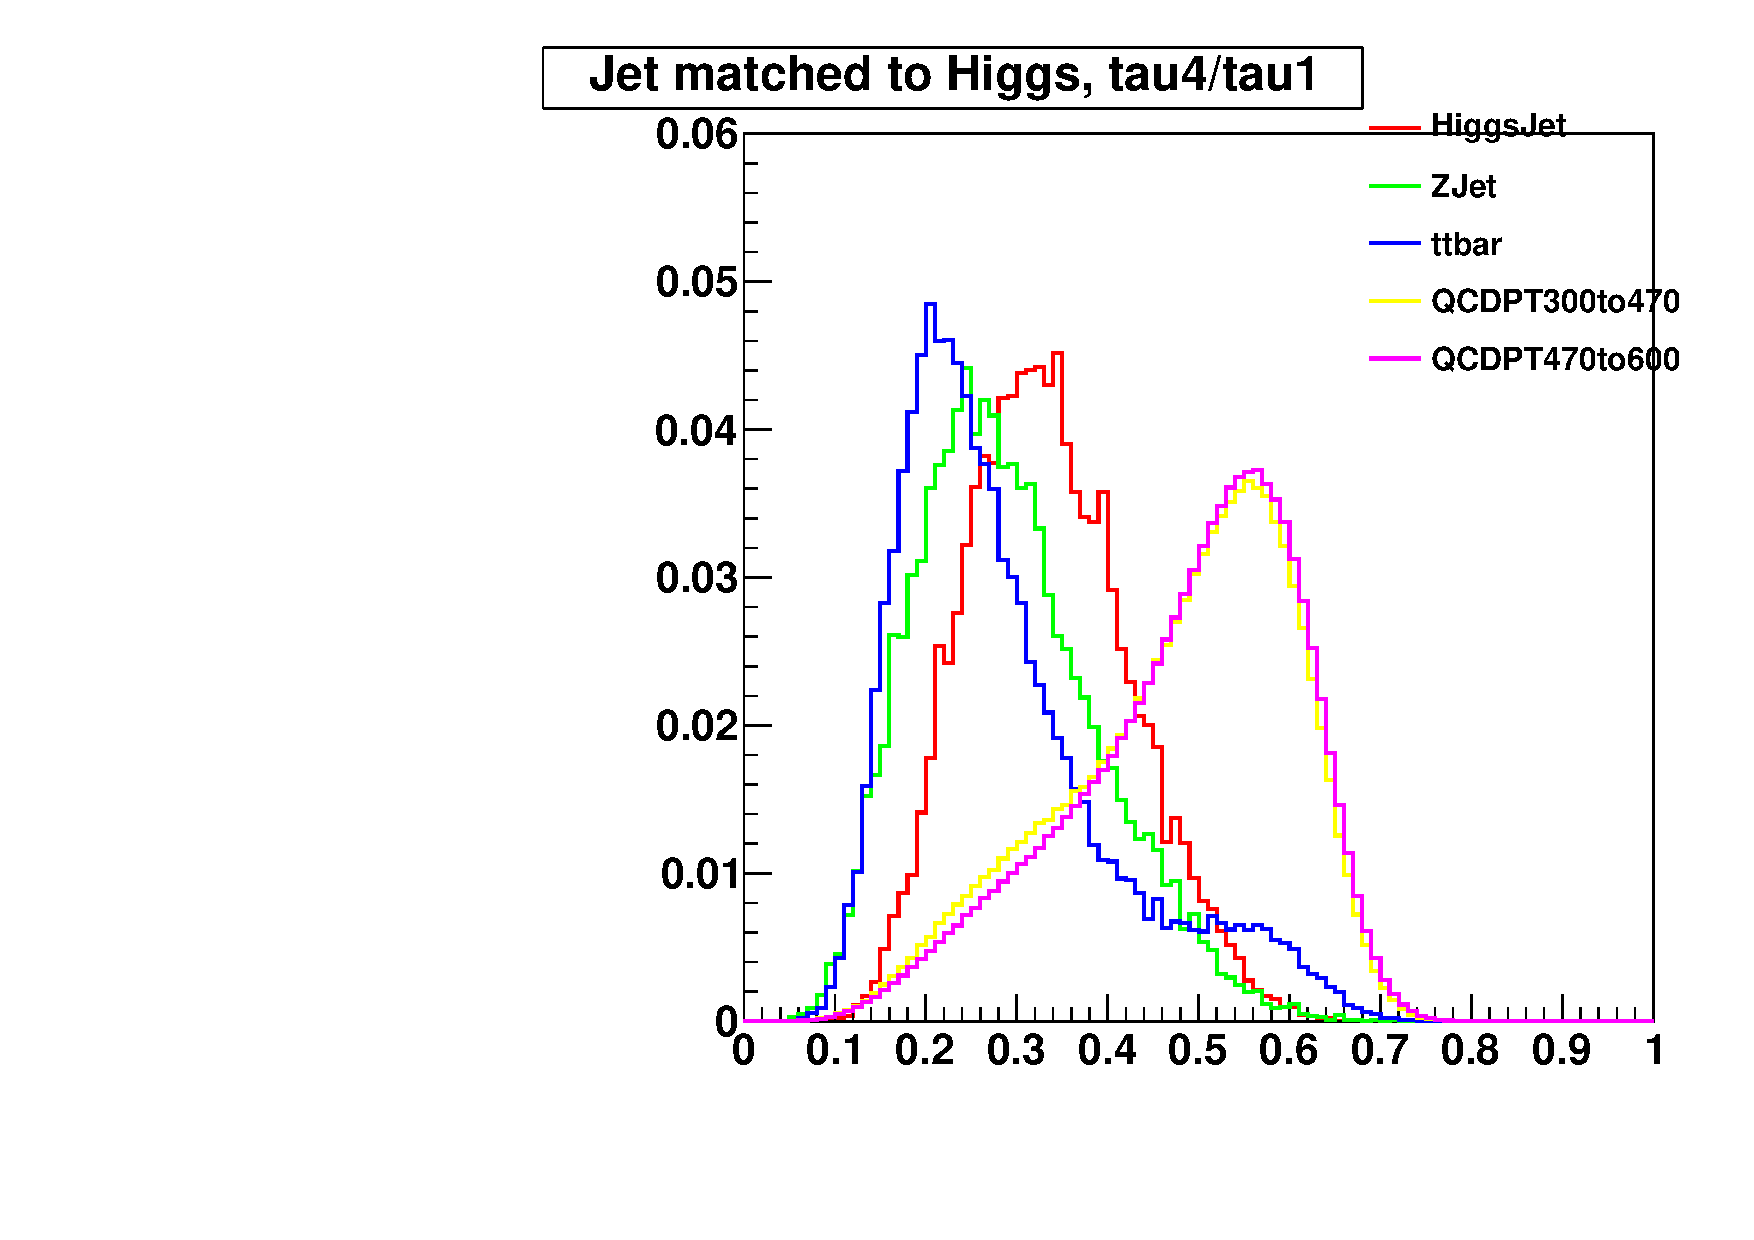
\includegraphics[width=0.49\textwidth]{HqqqqZqqfigs/tauNM/Tau41Pre.pdf}
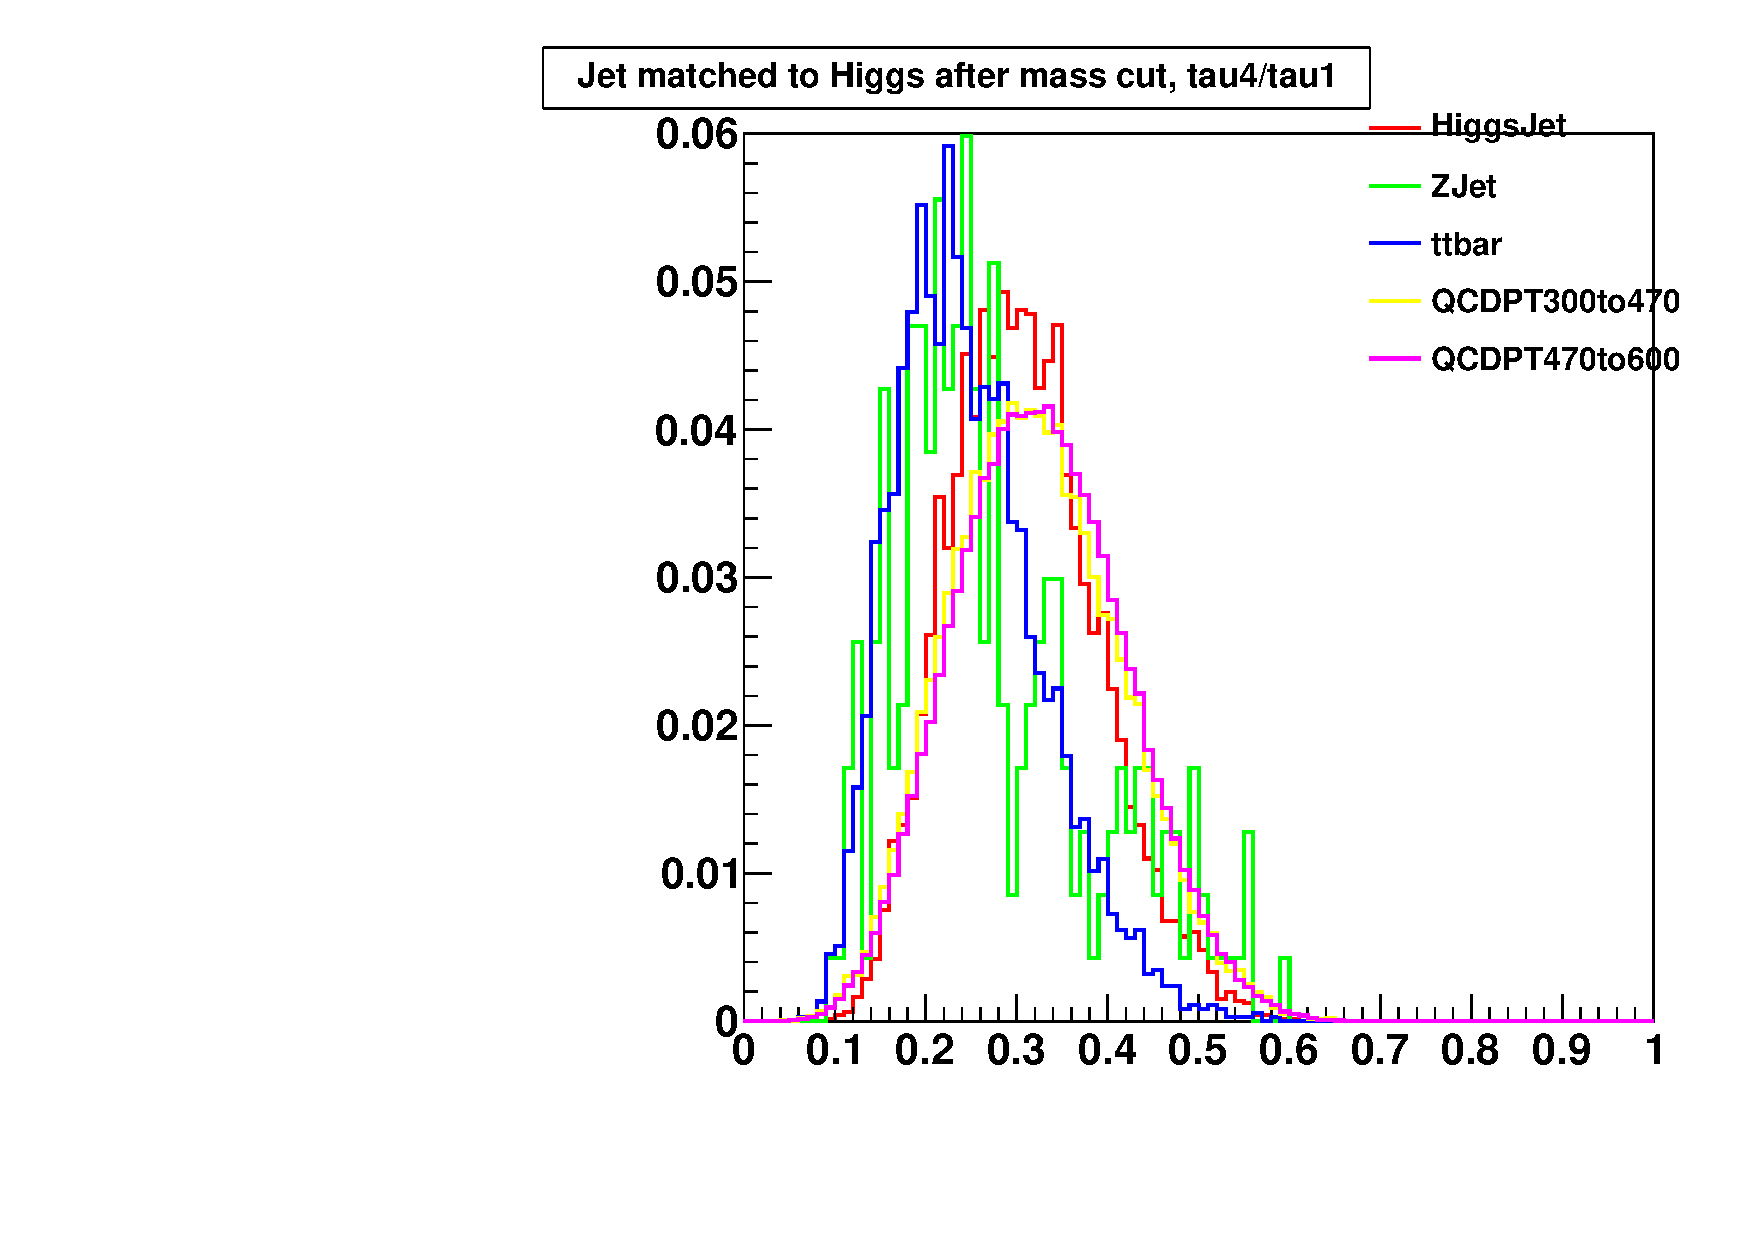
\includegraphics[width=0.49\textwidth]{HqqqqZqqfigs/tauNM/Tau41After.pdf}
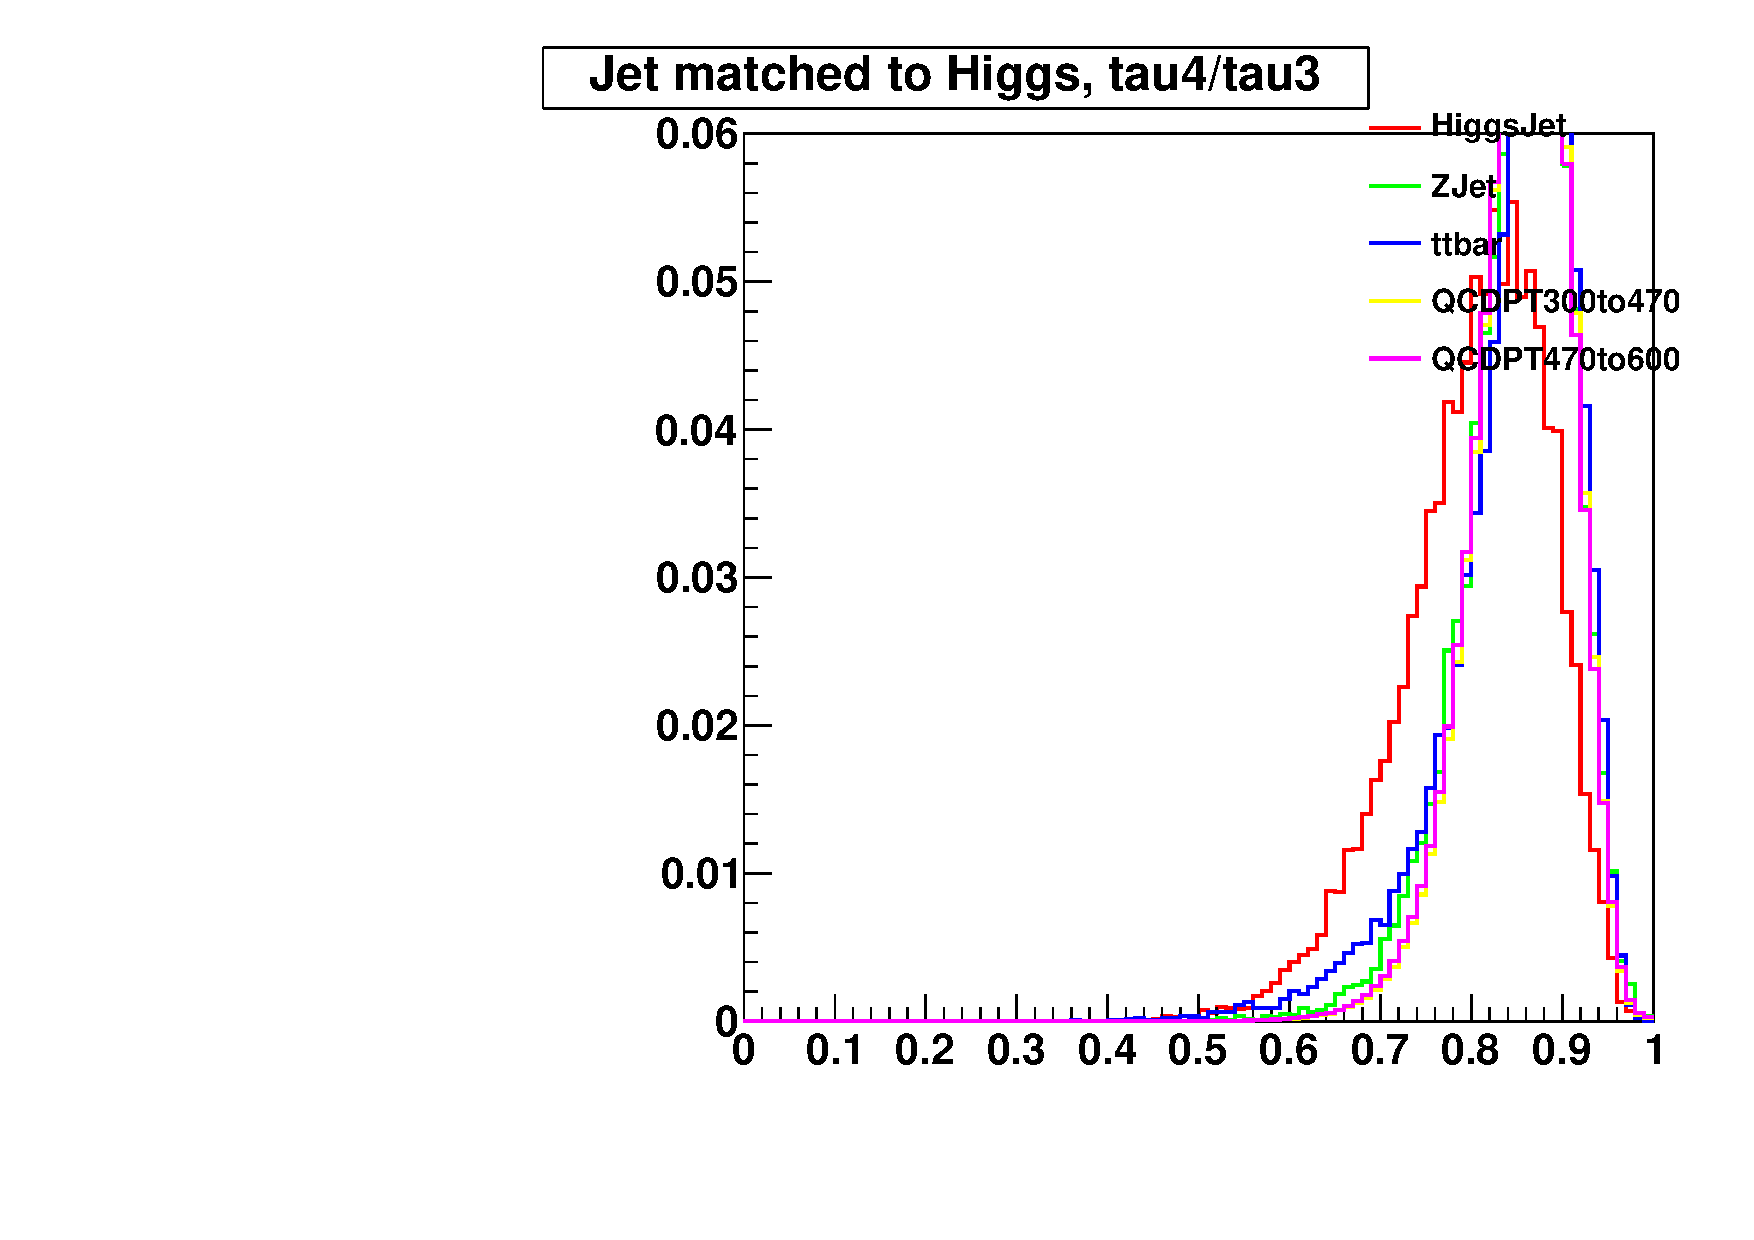
\includegraphics[width=0.49\textwidth]{HqqqqZqqfigs/tauNM/Tau43Pre.pdf}
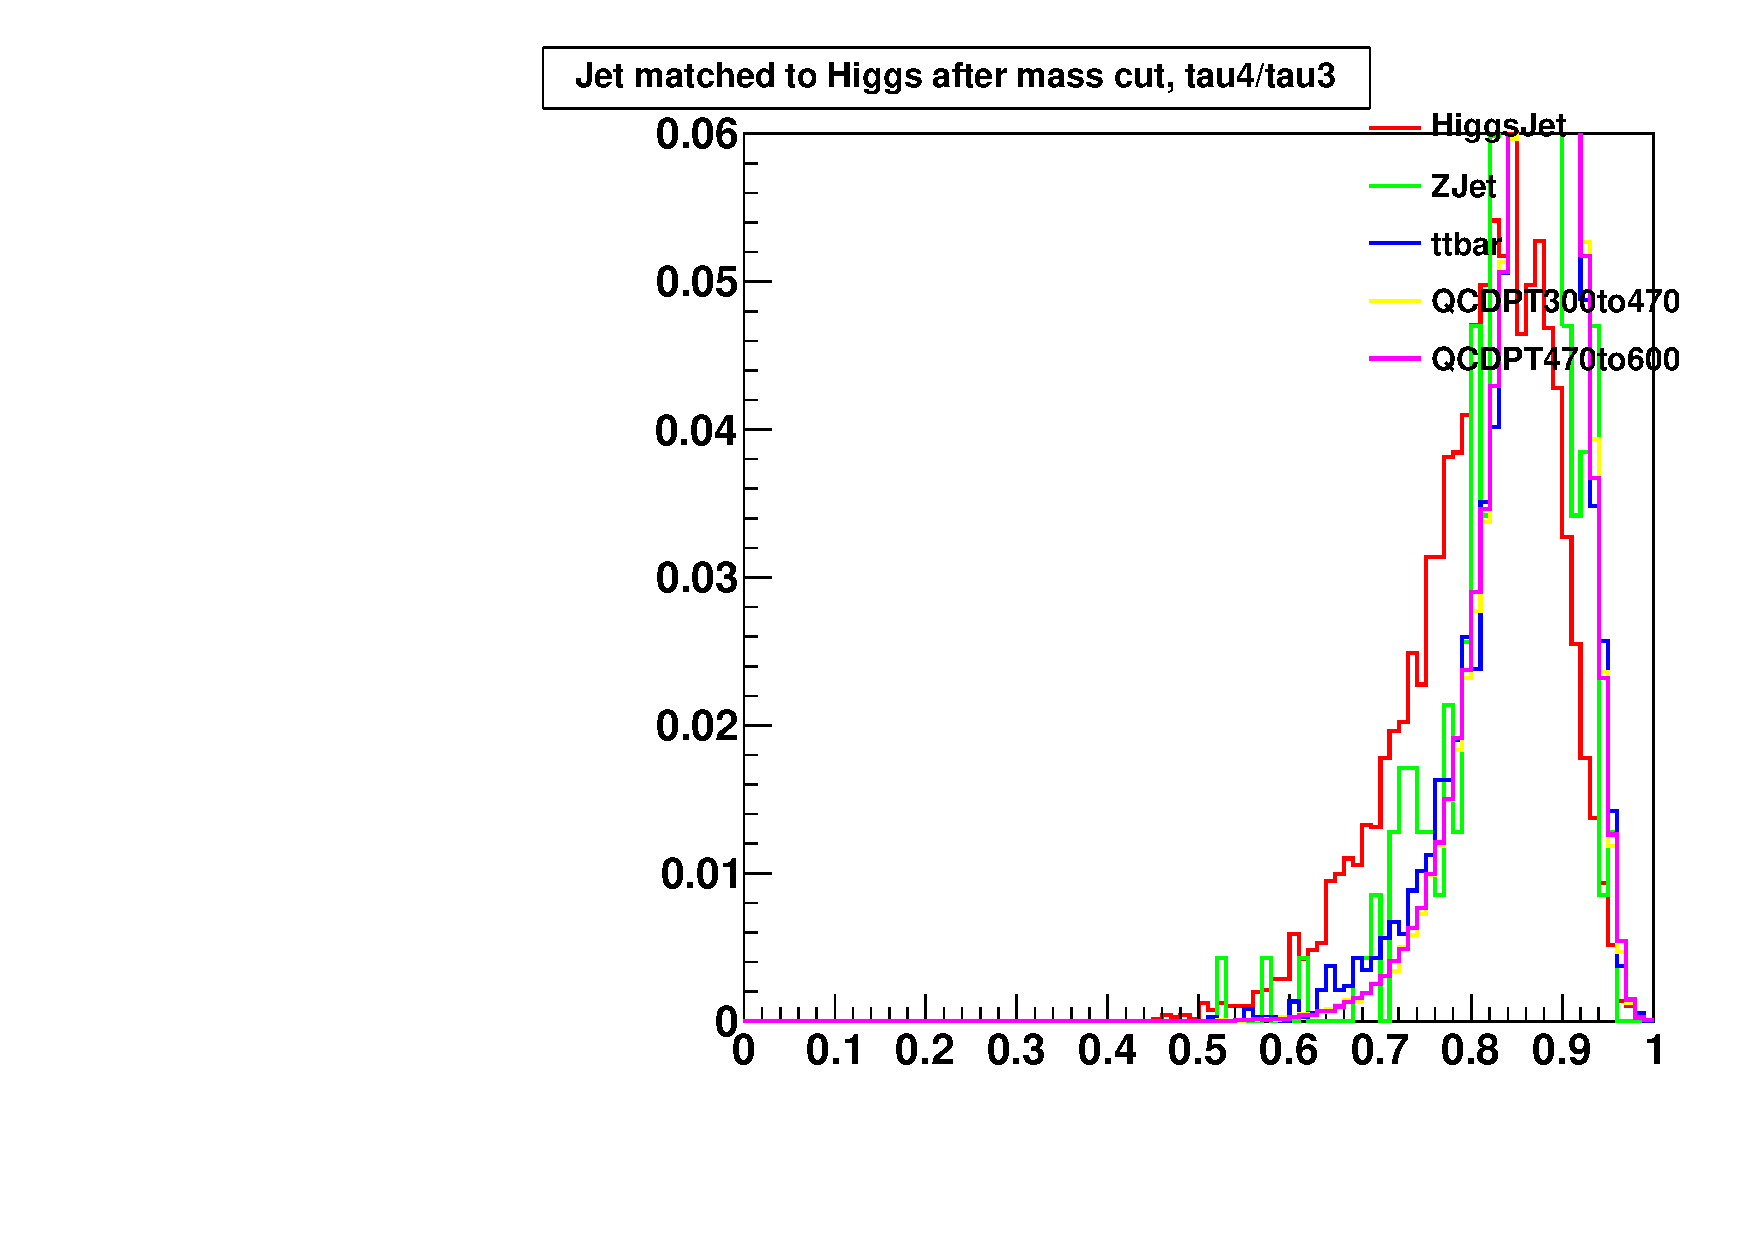
\includegraphics[width=0.49\textwidth]{HqqqqZqqfigs/tauNM/Tau43After.pdf}
\end{center}
\caption{
list of tauNM plots between Higgs genJet and Z genJet, hadronic top and QCD. 
Signal used is 2 TeV Z'. 
}
\label{fig:tauNM2}
\end{figure*}




\clearpage
